% Chapter4
\chapter{Implementierung} \label{chapter:thevetestcase}
\section{Modellierung der Anlage}
Für das Aufbauen einer Anlage, ist ein vorab überlegtes Konzept von großer Bedeutung. Mittels des Rohr- \& Instrumentenfließschemas wird ein später noch des öfteren abgeändertes Abbild erstellt. Die in der Anfangsphase aufkommenden Änderungen ergeben sich angesichts der nur partiellen Implementierung der Anforderungen. Initial wird hoher Wert auf Redundanzen gelegt. Erst eine größere Anzahl an Bauteilen kann einen parallelen Ablauf mehrerer Arbeitsschritte ermöglichen. Durch die drei eingebauten Tanks und zwei Reaktoren, die mittels der drei Hauptleitungen verbunden sind, ist das Umfüllen zwischen zwei Tanks, sowie das gleichzeitige Befördern von Flüssigkeit vom dritten Tank in einen der Reaktoren möglich.\\

Die zwei Pumpen sind so platziert, dass bei einem eventuell auftretenden Defekt die andere Pumpe deren Aufgabe übernehmen kann. Arbeitsschritte können dadurch zwar nur noch sequentiell abgearbeitet werden, jedoch kommt es nicht gleich zu einem totalen Ausfall der Funktionalität der Anlage. Eine weitere Absicherung gegen möglich aufkommende Störfälle ist die Position der Tanks. Durch ihre Lokalisation an der höchsten Stelle der Apparatur besteht die Opportunität die Schwerkraft zu nutzen.\\

\begin{figure}[h!]
  \centering
  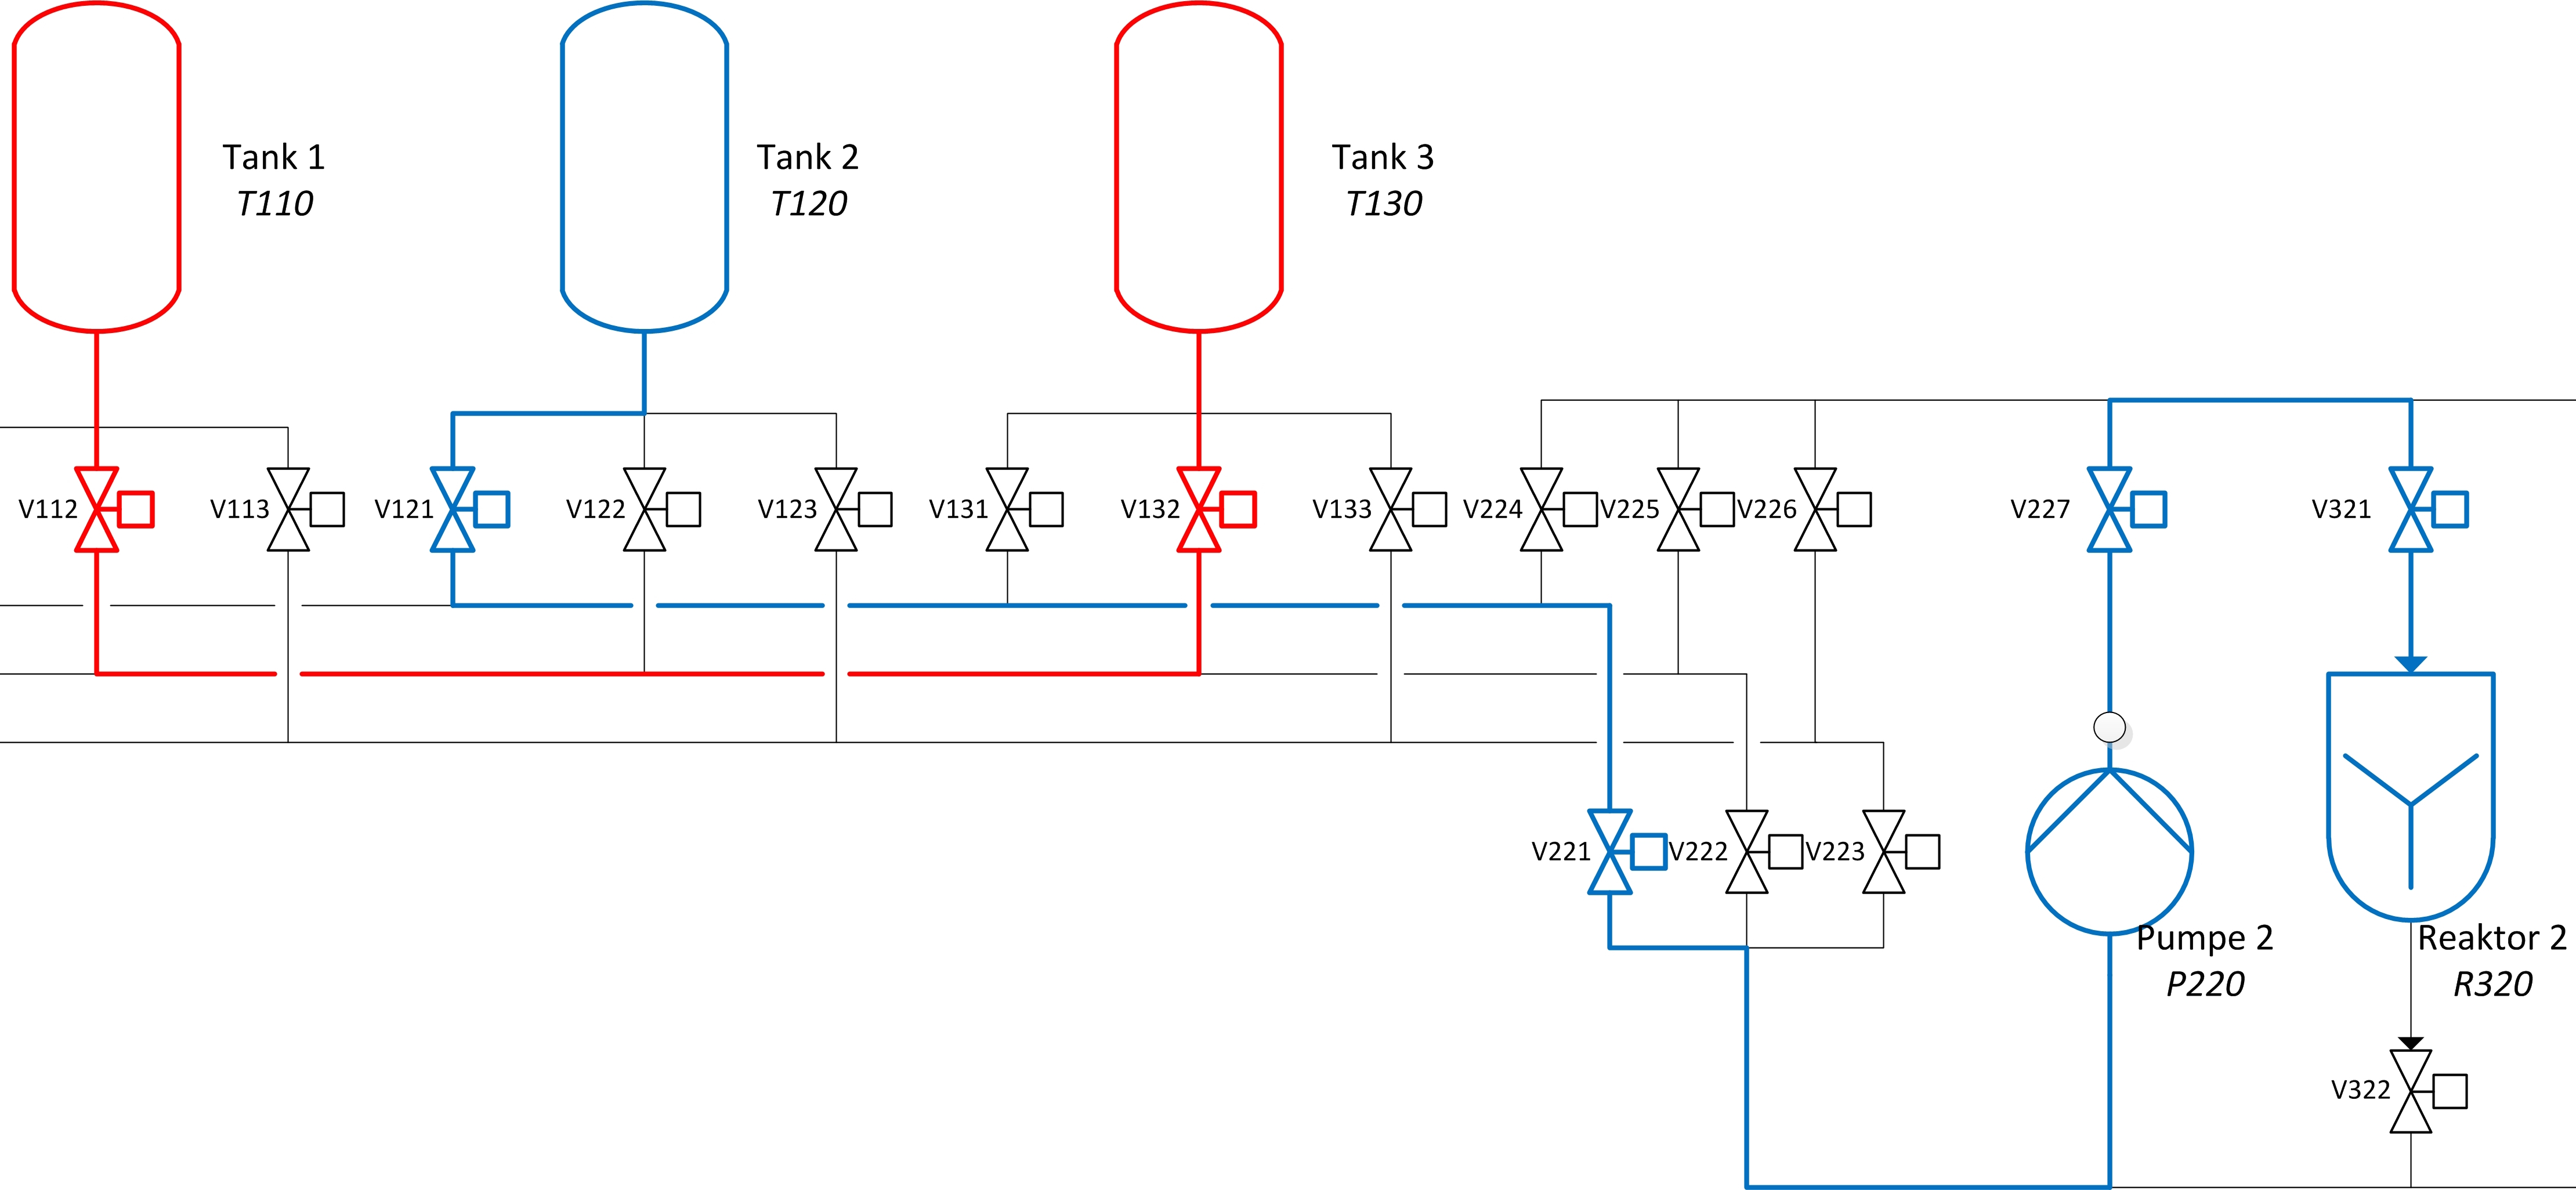
\includegraphics[width=1\textwidth]{graphics/implementation/RI_Impl_cropped.jpg}
  \caption{Mögliche Parallelität im RI ersichtlich}
\end{figure}

Jedes Ventil hat eine vorteilhafte Durchflussrichtung, die meistens mit einem Pfeil direkt auf dem Bauteil gekennzeichnet ist. Ganz abgesehen davon, ob es sich um ein Ventil handelt, welches im stromlosen Zustand geschlossen ist oder ob es ein schließendes Ventil ist, diese Vorgabe sollte stets eingehalten werden. Aspekte wie dieser haben in die Modellierung der Anlage selbstverständlich eingebaut zu werden.\\

\todo[inline]{BILD EINFÜGEN}

\begin{figure}[h!]
  \centering
  %\includegraphics[width=0.7\textwidth]{graphics/implementation/BILD}
  \caption{Ventil mit vorteilhafter Fließrichtung}
\end{figure}

Um in der Anlage befindliche Flüssigkeiten zu entfernen muss ein eigens für den Auslass vorgesehenes Ventil installiert werden. Vorteilhafterweise handelt es sich bei der Position dieses Bauteils um den tiefsten Punkt der Apperatur. Alternativ dazu kann dieses auch direkt nach einer Pumpe montiert werden.

\section{Aufbau der Anlage}
Auf Basis des Rohr- \& Instrumentenfließschemas kristallisiert sich eine exakte Anzahl an benötigten Bauteilen heraus. Für den noch bevorstehenden Aufbau der Anlage ist zu beachten, dass beim Auswählen der Einzelteile alles kompatibel sein muss. Nicht vorhandene Vereinbarkeit kann vor allem für diesen speziellen Anwendungszweck zu katastrophalen Auswirkungen führen, da einerseits mit Flüssigkeiten gearbeitet wird, sowie gleichzeitig stromdurchflossene Leitungen existieren. Eine Verbindung dieser genannten Komponenten hätte irreparable Schäden zur Folge. Im Rahmen einer übergeordneten Forschungsarbeit wurde diesem Projekt ein Budget von 6000 \euro \space zugesprochen. Die Auswahl der benötigten Teile hat verständlicherweise im Rahmen dieser beschränkten Geldmittel zu geschehen.\\
	
	Für einige von uns verwendete Element gibt es spezifische Parameter, die auf jeden Fall einzuhalten sind:\\
	
	\textbf{Ventile:}\\
	Ein ausschlaggebendes Kriterium der verwendeten Ventile ist, dass sie in stromlosem Zustand geschlossen sind. Im Falle eines Ausfalls der Energieversorgung kann somit sichergestellt werden, dass sich alle Verbindungen aus Schutz vor der Flüssigkeitsverlust schließen. Für die Funktion der Nutzung der Schwerkraft zum Umleiten von Flüssigkeiten ist auch relevant, Ventile zu haben, die keinerlei Vordruck benötigen, um den Durchfluss zu gewähren.\\

	\textbf{Tanks:}\\
	Abgesehen von einem für Testzwecke vernünftigen Füllvolumen ist es erforderlich einen Tank zu wählen, dessen Ausgang sich am niedrigsten Punkt befindet. Andernfalls kann man nur bedingt Nutzen aus der Schwerkraftsteuerung ziehen.\\
	
	\textbf{Pumpen:}\\
	Mit Hilfe eines Gleichstrom - Wandlers muss es möglich sein, die Pumpen mit dem zur Verfügung stehenden Ausgangstrom der SPS von 0 - 10 Volt zu betreiben.\\
	
	\textbf{Rohre:}\\
	Die Rohre müssen jedenfalls dem Druck der Pumpen standhalten können. Desweiteren ist das exakt abzustimmende Einpassen in die Ventile, um Dichte gewährleisten zu können, ein wichtiger Parameter.\\

	Die bereits bei der Bestellung bekannten, tatsächlichen Maße der Bauteile, haben einen relevanten Einfluss auf den finalen Aufbau. Da es auch bei der Profilplatte physikalische Grenzen gibt, muss die endgültige Positionierung genauestens überlegt ausfallen. Der zukünftigen Vereinfachung des Aufbaus der Produktionsanlage halber, wurde daher projektintern beschlossen, ein kleines Modell der Apparatur zu erstellen. Da aus dem Rohr- \& Instrumentenfließschema keinerlei Information zur endgültigen Lokalisation der Bauteile ersichtlich ist, wird ein erster physikalischer Entwurf konstruiert. Mit Hilfe diesem können Abstände zueinander stehender Elemente deutlich gemacht werden. Realisiert wird der genannte Prototyp mit leicht zugänglichen Arbeitsmaterialien wie etwa Trinkhalme, Papier und Klebeband.\\
	
		\todo {Bild des Miniaturmodells}

	Für den tatsächlichen Aufbau ergibt sich günstigerweise die Möglichkeit, mechanische Anforderungen mit Hilfe der technischen Werkstätte abzuwickeln. Profilschienen, die als stabilisierendes Gerüst dienen, werden penibelst mit der Aluminiumsäge auf das gewünschte Maß geschnitten. Im späteren Verlauf werden diese samt den Tanks zum ersten aufgebauten Teil der Anlage. Für die Verbindung der Tanks, Pumpen, Ventile und Reaktoren dienen undurchsichtige Kunststoffrohre. Um gewährleisten zu können, dass die Verbindung absolute dicht ist, müssen die Rohre unbedingt gerade geschnitten sein. Abermals dürfen dafür Maschinen der mechanischen Werkstatt verwendet werden. Erst mit einer Bandsäge grob vorgeschnittene Rohrstücke werden in eine konventionelle Drehmaschine eingespannt. Mit einem scharf angeschliffenen Drehstahl ist es möglich, den unsauberen Schnitt absolut plan zu gestalten. Nachdem abschließend einzelne Komponenten noch entgratet werden, ist die Arbeit an den Rohren zur Verbindung getan.\\
	
		\todo{Bild: Erster Aufbau (Tanks, Hauptpipes)}
		
		TODO ... weitermachen

\section{Phasen und Rezepte}
\section{HMI}
Für dieses Projekt wurde als SCADA System die Software zenon vorgegeben, daher wurde das HMI in zenon Supervisor (zenons HMI Programm) umgesetzt.\\
\\
\textbf{Visualisierung}\\
In zenon wird eine Visualisierung  \glqq Bild\grqq\space  gennant. Dieses kann man mit vorgefertigten Elementen erweitert werden. 

Als Ausgangspunkt für die Visualisierung wurde das RI-Fließeschema zur Hand genommen. Von diesem wurde die Anzahl der Elemente und die Grundstruktur übernommen. Als nächsten Schritt musste evaluiert werden, welche Inhalte des RI-Fließschemas für die Visualisierung relevant und welche Informationen nicht vorhanden waren.
\begin{description}
\item[Wichtige Elemente]~\par
	\begin{itemize}
		\item Rohre in Verwendung kennzeichnen
		\item Sensorwerte anzeigen
		\item ....ADD MORE
	\end{itemize}
\end{description}
%todo add image
ABBILDUNG\\

\textbf{Feldbuskonfiguration}\\
Um eine Visualisierung mit aktuellen Sensorwerten zu befüllen, wird eine Verbindung zur SPS benötigt. In zenon wird eine Verbindung über zenon Logic (im weiteren nur noch Logic genannt) hergestellt.\\
\\
Als ersten Schritt, um in Logic eine SPS hinzuzufügen, musste im Unterpunkt \glqq Feldbuskonfiguration\grqq\space die Treibersoftware für die ADAM5550 SPS hinzugefügt werden. Darauf hin wurden alle Module, die an der SPS angebracht wurden, in dieser Konfiguration hinzugefügt.\\%todo Position
\begin{figure}[h!]
  \centering
  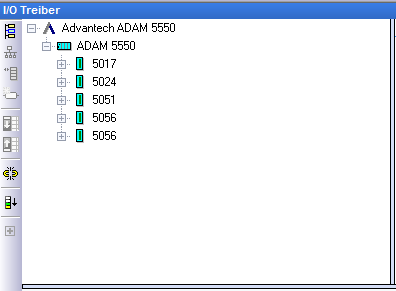
\includegraphics[width=0.7\textwidth]{graphics/implementation/Feldbuskonfiguration}
  \caption{Feldbuskonfiguration}%todo Grafik name
\end{figure}
\\
\textbf{Variablen}\\
In zenon können auf mehrere Arten Variablen erstellt werden, damit diese jedoch für die Visualisierung und von Logic sichtbar sind, müssen sie als Globale Variable definiert werden. Der einfachste Weg dafür ist es, im Logic Variablenfenster über den Reiter  \glqq Globale Variablen\grqq\space  die Funktion  \glqq Variable hinzufügen\grqq\space  aufzurufen.\\%todo Position
\begin{figure}[h!]
  \centering
  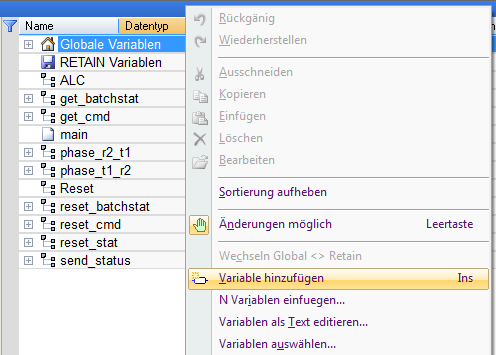
\includegraphics[width=0.7\textwidth]{graphics/implementation/Variablen}
  \caption{Variablen}%todo Grafik name
\end{figure}\\
Nachdem alle Variablen erstellt wurden, müssen diese mit der Feldbuskonfiguration verknüpft werden. Durch diesen Schritt erhält man Zugang zu den an der SPS angeschlossenen Elementen.\\
Die erstellten Variablen mussten als nächstes in der Visualisierung eingetragen werden um in dieser im nächsten Schritt eine Steuerung zu erzeugen.\\
\\
%Feldbuskonfiguration -> Konfiguration einfügen (Advantech ADAM 5550) -> Master/Port hinzufügen (ADAM 5550) -> Slave/Datenblock einfügen (Slot:Steckplatz an SPS; Module: Analog/Digital|In/Out|4/8/16 Channels...) -> Variable hinzufügen (Channel; Variablenname)
%Variable -> Globale Variable hinzufügen (erzeugt Variable in logic und auch im supervisor zugänglich für die Visualisierung) -> In Visualisierung zu den Elemente die richtigen Variablen hinzufügen -> Bei Feldbbuskonfiguration bei richtiger I/O auf richtigem Channel hinzufügen
%TEST -> logic Programm hochladen -> Variablen in logic zeigen aktuelle werte an -> check mit werten direkt von der SPS

%Umrechnen von Sensorwerten: 
%Durchflusssensor Digital -> etwa 900 ticks pro Liter -> Timer bid 900 ticks -> Liter/min
%Füllstandsensor 4-20mA -> 4=voll, 20=leer -> Variablen/Tank Konfiguration -> Umrechnung 4=100, 20=0
%Ventilstatus 0/1 -> Variablen Konfiguration -> Extremwerte farblich markieren -> Ventil Elementfarbe nach Variablen Farbe
\textbf{Steuerung}\\
Phase 1 Steuerung mittels Buttons\\
	Der erste Versuch war es die Steuerung mittels einfachen Buttons umzusetzen. Diese haben meist die in zenon vorhandene Funktion  \glqq Sollwert absetzen\grqq\space  verwendet, welche den Wert einer Variable ändert.\\
	So konnten alle Funktionen umgesetzt werden, dadurch erhielt das  \glqq Bild\grqq\space  jedoch viele Elemente die von der Eigentlichen Visualisierung ablenkten.\\
\\
Phase 2 Versteckte Buttons\\
	Um den Element-Overload zu verringern war der nächste Schritt die Button zu  \glqq verstecken\grqq\space  indem sie Transparent über die eigentlichen Elementen (beispielsweise ein Ventil) verschoben wurden.\\
	In der Visualisierung wurden nun weniger  \glqq unwichtige\grqq\space  Bausteine angezeigt, die Elemente waren jedoch immer noch da, wodurch die Größe (MB) der Visualisierung deutlich anstieg.\\
\\
Phase 3 Funktionale Elemente\\
	Der nächste schritt war es die nicht funktionalen Grafikelemente durch Buttons in Form der gewünschten Elemente zu ersetzten.\\
\\
\textbf{Rezepterstellung}\\

\section{Ontology}
\section{Aktivitätsdiagramm}
\section{Codegenerierung}

TODO